\chapter{Энергонезависимая память на основе сегнетоэлектрических материалов}\label{ch:ch0}
\section{Флеш-память}\label{sec:ch0/sec1}
На момент написания этой работы доминирующим на рынке видом энергонезависимой памяти (NVM) является флеш-память. Основным компонентом флеш-памяти является транзистор с плавающим затвором (рис. \cref{fig:floating_gate_transistor}). При приложении потенциала к управляющему затвору происходит туннелирование электронов сквозь диэлектрической слой, что приводит к инжекции заряда в плавающий затвор. При отсутствии напряжения ток через потенциальный барьер значительно уменьшается, тем самым обеспечивая длительное хранение заряда в плавающем затворе, а значит и долгий срок хранения информации в устройстве. При считывании проводимость канала транзистора определяется наличием заряда на затворе: в отсутствии заряда ток протекает, а при наличии заряда канал остаётся закрытым.

\begin{figure}[ht]
    \centerfloat{
        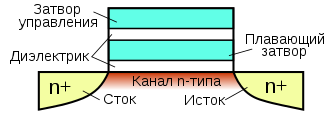
\includegraphics[scale=0.8]{floating_gate_transistor.png}
    }
    \caption{Транзистор с плавающим затвором}\label{fig:floating_gate_transistor}
\end{figure}

Стоит отметить, что в большинстве современных устройств флеш-памяти используются многобитовые ячейки памяти (multi-level cell), которые позволяют увеличить объём хранимой информации за счёт увеличения количества различимых состояний заряда на затворе (\(2^N\) состояний соответствуют \(N\) битам памяти).

Для повышения объёма записи в данный момент преимущественно используется увеличение количества слоёв в устройстве с помощью перехода к изготовлению трёхмерных интегральных микросхем (3D IC) и 3D V NAND...

Потенциально большая скорость
Открывают ряд преимуществ
- Возможность создания универсальной памяти, сочетающей в себе быстрый доступ к информации и энергонезависимость
- Потенциально неограниченное количество циклов перезаписи
- Потенциально большая скорость

\section{Сегнетоэлектрическая память}\label{sec:ch0/sec2}
\subsection{Сегнетоэлектрики}
Сегнетоэлектричество (СЭ) "--- свойство материалов, позволяющее им обладать спонтанной поляризацией. То есть в отсутствии внешнего электрического поля в таких веществах сохраняется ненулевой вектор поляризации. Наличие этого свойства в материале определяется кристаллической решёткой. Так, СЭ может проявляться лишь в таких пространственных группах (фазах) вещества, кристаллическая решётка (сингония) которых не является центросимметричной.

Одним из наиболее характерных свойств СЭ материалов является наличие петли гистерезиса в зависимости поляризации \(P\) от напряжённости электрического поля \(E\) (рис. \cref{fig:hysteresis}). Важные характеристики, которые часто используются при характеризации СЭ материалов: коэрцитивное поле и остаточная поляризация также отражены на рисунке \cref{fig:hysteresis} Стоит отметить, что зависимость такого вида может быть получена и в несегнетоэлектрических материалах за счёт зарядки/разрядки ловушек в диэлектрике, а значит не может быть использована как критерий проявления СЭ в материалах.

\begin{figure}[ht]
    \centerfloat{
        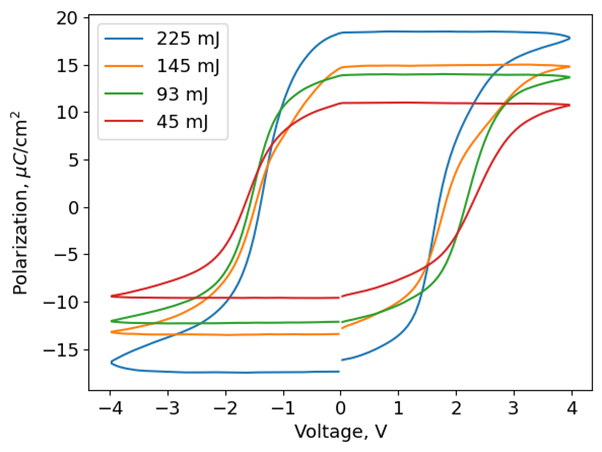
\includegraphics[scale=0.8]{hysteresis.png}
    }
    \caption{Зависимость поляризации \(P\) от напряжённости электрического поля \(E\) в сегнетоэлектрике}\label{fig:hysteresis}
\end{figure}

\subsection{Устройства памяти на основе сегнетоэлектриков}
Наличие двух стабильных состояний кристаллической решётки, которым соответствует положительная и отрицательная поляризация материала позволяет использовать сегнетоэлектрические материалы как функциональный слой в устройствах энергонезависимой памяти. Основные концепции сегнетоэлектрической памяти включают в себя коммерчески доступную сегнетоэлектрическую память с произвольным доступом (ferroelectric random access memory, FRAM), сегнетоэлектрический полевой транзистор (ferroelectric field-effect transistor, FeFET) и сегнетоэлектрический туннельный переход (ferroelectric tunnel junction, FTJ), принципиальная схема которых отражена на рисунке \cref{fig:fram}.

\begin{figure}[ht]
    \centerfloat{
        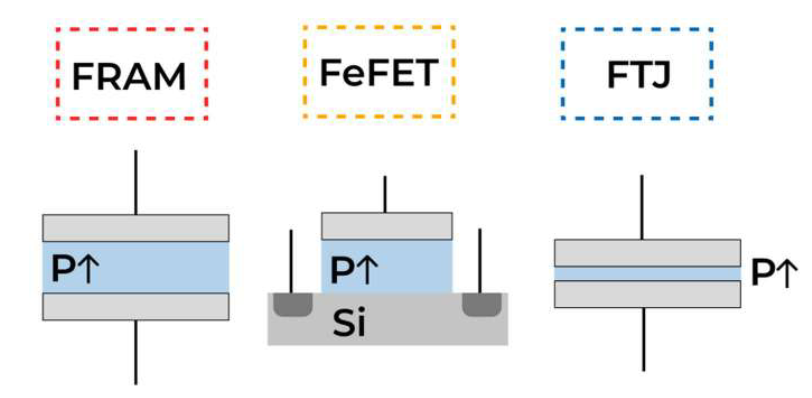
\includegraphics[scale=0.8]{FRAM.png}
    }
    \caption{Схема сегнетоэлектрической памяти}\label{fig:fram}
\end{figure}

\FloatBarrier
